\chapter{Quick Start} \label{chap:quickstart}
%==================================================================
%================== PRIMERA SECCIÓN ===============================
%==================================================================
\section{Installing Magentix2} % Desktop Edition}
%This distribution is based on C++ implementation for the Qpid message broker and supports all features of Magentix2, it is recommended both for developers and end-user applications.
%This installation is offered only for Ubuntu Linux version. In order to use in other systems please refer to section \ref{sec:InstallMagentix2JavaBased}.
\subsection{Requirements}
\begin{itemize}
\item Oracle Java Development Kit (JDK) 7 or later\footnote{\url{http://www.oracle.com/technetwork/java/archive-139210.html}}. %Donde este explicado que hace falta java, exactamente no se que secci�n es.
\item Apache Tomcat 7 or later\footnote{\url{http://tomcat.apache.org/download-70.cgi}}
\item MySQL server 5.0 or later\footnote{\url{http://www.mysql.com/downloads/}}
\end{itemize}


\subsection{Installation of Magentix2}

In order to install Magentix2,  the corresponded zipped package must be downloaded\footnote{The latest installable version is in: \url{http://gti-ia.upv.es/sma/tools/magentix2/downloads.php}}. Once Magentix2 is downloaded, you need to unzip the file. Just double-click the file or run the following command:

\texttt{\$ unzip magentix2-\MagentixVersion.zip}

In the unzipped directory you have now the Magentix2 agent platform\texttrademark ready to be configured and started. Before running the Magentix2 platform you need to finish the installation by executing the setup script.
\begin{itemize}
    \item In Linux and MacOS X run the following command:
        \begin{verbatim}
$ ./magentix-setup.py
        \end{verbatim}
    \item In Windows XP, Windows 7 and Windows 8 double-click the \texttt{magentix-setup.exe} file.
\end{itemize}


Then, a text interface for the installation is provided. This setup process will ask you some required users and passwords to configure and deploy the components needed by Magentix2. It will also check taht all the required dependencies are installed and properly configured. The setup script will ask you for the following data:
\begin{itemize}
    \item MySQL root password: used to create the magentix user and create the database schema for the platform.
    \item Tomcat user and password: used to deploy the Magentix webservices to the tomcat app server. Note that the tomcat user \textbf{MUST} have the \texttt{manager-script} role to be able to deploy webapps. To do this add the following lines to your \texttt{tomcat-users.xml} file (located where your tomcat installation is or at \texttt{/etc/tomcat}), where USERNAME and PASSWORD must be changed by the user and password you assign to tomcat:
    \begin{verbatim}
<role rolename="manager-script"/>
<user username="USERNAME" password="PASSWORD" 
                          roles="manager-script"/>
    \end{verbatim}
    
\end{itemize}

If every dependency is correctly installed and running the setup script will finish with the message: 
\begin{center}
\texttt{"Magentix succesfully installed."}
\end{center}

When installation ends, you can run the Start-Magentix script in order to start the services and platform agents. this script must be executed as follows:

\begin{itemize}
    \item In Linux and MacOS X run the following command:
\begin{verbatim}
$ ./Start-Magentix.sh
\end{verbatim}
    \item In Windows XP, Windows 7 and Windows 8:
\begin{verbatim}
> Start-Magentix.bat
\end{verbatim}
\end{itemize}

To check that all is correctly configured and Magentix2 has been successfully installed and running, execute the example Start-BasicExample.sh.
This script must be executed as follows:

\begin{verbatim}
$ cd  examples
$ ./Start-BasicExample.sh
\end{verbatim}

The output of this example should be like the following one:

\begin{codigo}
 Executing, I'm consumer
2010-12-13 13:07:48,364 INFO  
[Thread-2] SingleAgent_Example.SenderAgent2 (?:?) - 
        Executing, I'm the sender
Executing, I'm the sender
Mensaje received in consumer agent,
 by receiveACLMessage: Hello, I'm the sender
HearderValue
\end{codigo}



\subsection{Magentix2 installation description}\label{sec:InstallMagentix2DistDirectory}
Once Magentix2 has been installed, the following folders are created:
\begin{itemize}
\item \textbf{/} magentix root directory: 
 includes the executable files and folders required to launch and start the platform and services. The main ones are the following, which allows users to start and stop the Magentix2 platform:

    \begin{itemize}
         \item \textit{Start-Magentix.sh} and \textit{Start-Magentix.bat}: it launches the Qpid server and the platform agents (OMS, SF, TM and bridge agents).  %%\footnote{Magentix2 is launched without security, to enabled security refer to section \ref{sec:DesktopWithSecurity}}. 

        \item \textit{Stop-Magentix.sh} and \textit{Stop-Magentix.bat}: it stops Qpid and the platform agents (OMS, SF, TM and bridge agents). The commands needed to execute this script are:
        \begin{verbatim}
$ ./Stop-Magentix.sh
        \end{verbatim}

        \item \textit{LICENSE.txt}: includes the license under Magentix2 is distributed. Magentix2 is licensed under the GNU LESSER GENERAL PUBLIC LICENSE\footnote{\url{http://www.gnu.org/copyleft/lesser.html}}.
        \item \textit{RELEASE\_NOTES}: includes the changelog of the last releases of the platform.
        \item \textit{magentix-setup.py} and \textit{magentix-setup.exe}: configure magentix to be launched at first time.
    \end{itemize}

\item \textbf{configuration/} sub-directory: includes the Settings.xml and loggin.xml configuration files, necessary to launch Magentix2 user agents.

%%\item \textbf{security/} sub-directory: includes all required files to launch Magentix2 in secure mode. 
 
\item \textbf{docs/}
 includes the API in html format and the Magentix2 User manual in pdf format.
\item \textbf{lib/}
 includes Magentix2 library an all additional libraries required by Magentix2. How to import this library in projects is showed in  section \ref{sec:devel1stAgent}.
\item \textbf{examples/}
 includes some examples of Magentix2 agents implementation.
\item \textbf{src/}
 includes Magentix2 sources.
\item \textbf{webapps/}
 includes all services required by \textsc{Thomas} and Magentix2. It also includes a user web service example. 
 \item \textbf{bin/}
  includes some executables needed by Magentix2 to run.
\end{itemize}


\subsection{Unistalling Magentix2}

Magentix2 is very simple to remove from one system. The steps to uninstall are:
\begin{enumerate}
\item Stopping Magentix2 platform.
\begin{verbatim}
$ ./Stop-Magentix.sh
\end{verbatim}
\item Deleting Magentix2 installation directory.
\end{enumerate}


%==================================================================
%================== SEGUNDA SECCIÓN ===============================
%==================================================================
\section{Developing and executing a first agent}\label{sec:devel1stAgent}
This section explains step by step how to program a Magentix2 agent. The images shown here correspond to the Eclipse IDE, but everything should be similar in any other IDE. Magentix2 library works with jdk1.7 which is available at: \url{http://www.oracle.com/technetwork/java/javase/downloads/index.html}

The first step is to start Eclipse and create a new project (MyFirstAgent). The java library \texttt{magentix2-\MagentixVersion-jar-with-dependencies.zip} has to be included in the project as a referenced library. Magentix2 platform and the agents running on it need a configuration folder with two files: \texttt{Settings.xml} and \texttt{loggin.xml}. \texttt{Settings.xml} configures all the parameters related to the platform functionality, like MySQL parameters or how agents connect to the QPid broker. \texttt{Loggin.xml} is the configuration file for the Magentix2 logger, where is specified how log messages are displayed. Magentix2 uses log4j as debugger, for more information about this software, please, refer to: \url{http://logging.apache.org/log4j/1.2/manual.html}. 

There is a valid configuration folder for any Magentix2 project in the Magentix2 installation folder. In this example project, this configuration folder will be used. Thus, it is only necessary to copy the folder \verb|configuration/| in the root folder of the project (in this case \verb|/workspace/MyFirstAgent/}|). Then, it is necessary to create a new package named \textit{agent} in the project. In figure \ref{img:develop1} it is shown how Eclipse looks like after taking these actions.
\begin{figure}[!h]
\centering
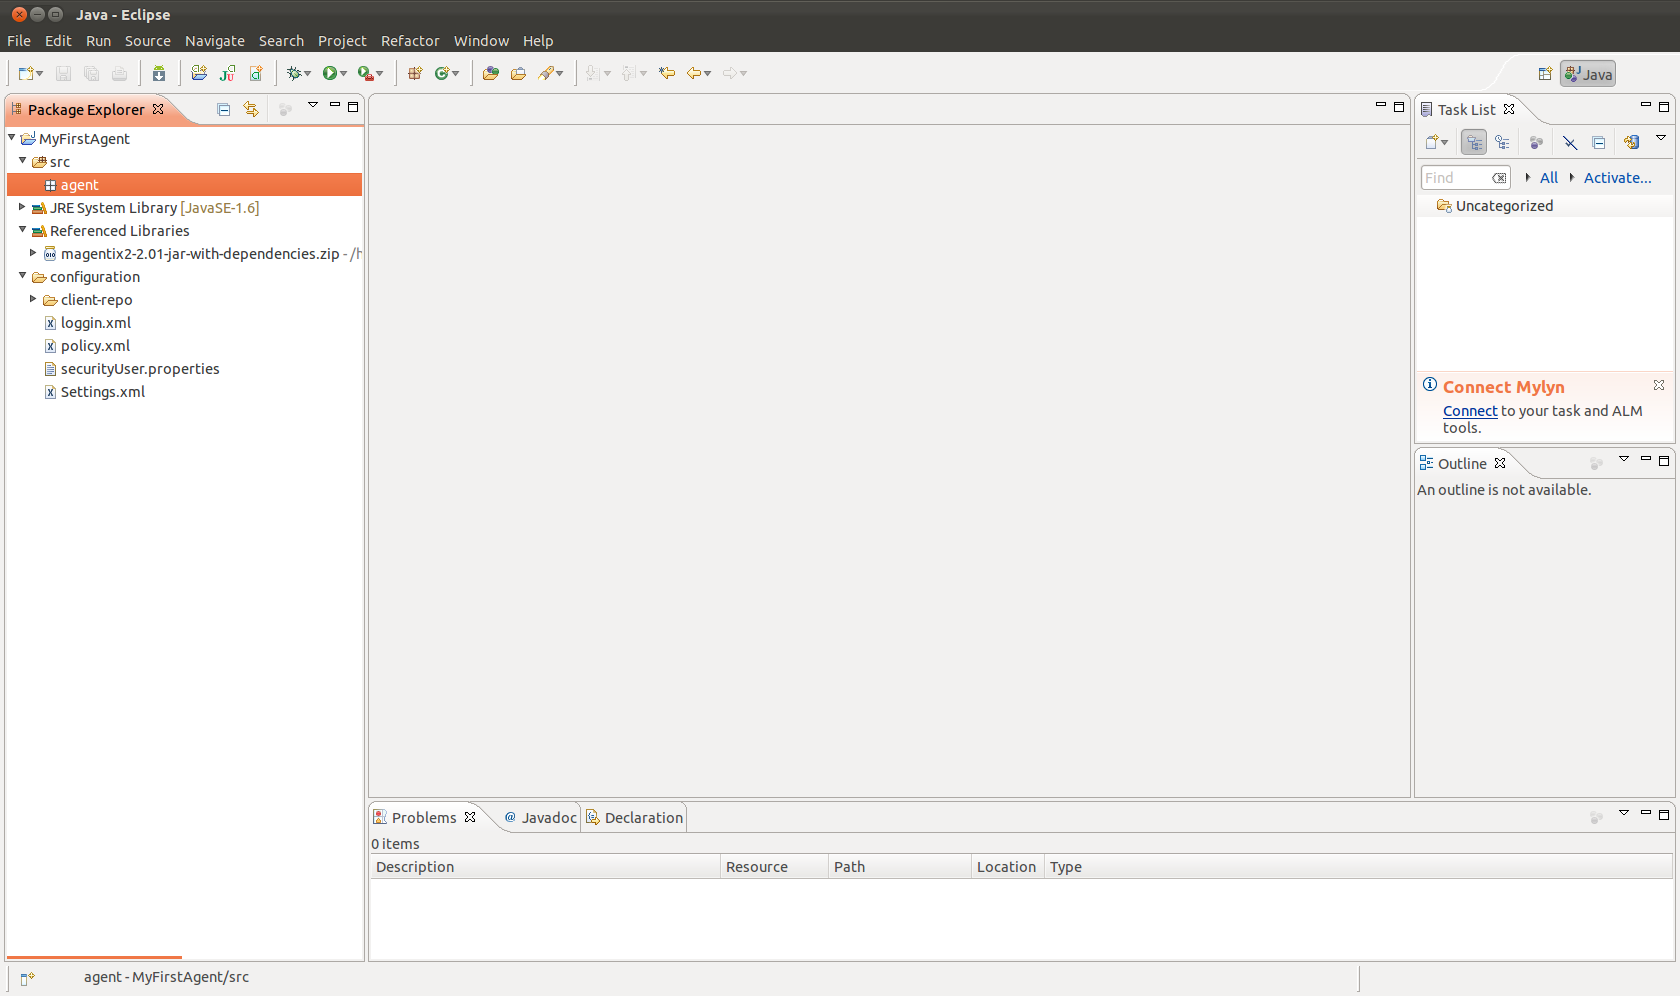
\includegraphics[scale=0.25]{Quickstart/images/develop1}
\caption{Project and package creation}
\label{img:develop1}
\end{figure}

The example shown here consists in two agents: \textit{Sender} and \textit{Consumer}. The agent \textit{Sender}  sends a message to agent \textit{Consumer}, who  writes the content of the received message on the console. In order to set this example, it is required to create three Java classes: Sender.java, Consumer.java and Main.java. Sender.java and Consumer.java will contain the code of the agents. Besides, Main.java will create the connexion to the broker for the agents and start them.

Now, how to program the Sender.java class is shown. This class has to extend BaseAgent class (section~\ref{sec:BaseAgent}). Therefore, it is necessary  to import some classes from magentix2-\MagentixVersion-jar-with-dependencies.zip. Once the library is included, Eclipse suggests you to import the necessary classes that library. Figure \ref{img:develop2} shows Sender.java at that moment. As it can be seen in the figure, the code of the agent has an error because it lacks a constructor. So, a basic constructor which calls the constructor of the base class is created.

\begin{figure}[!h]
\centering
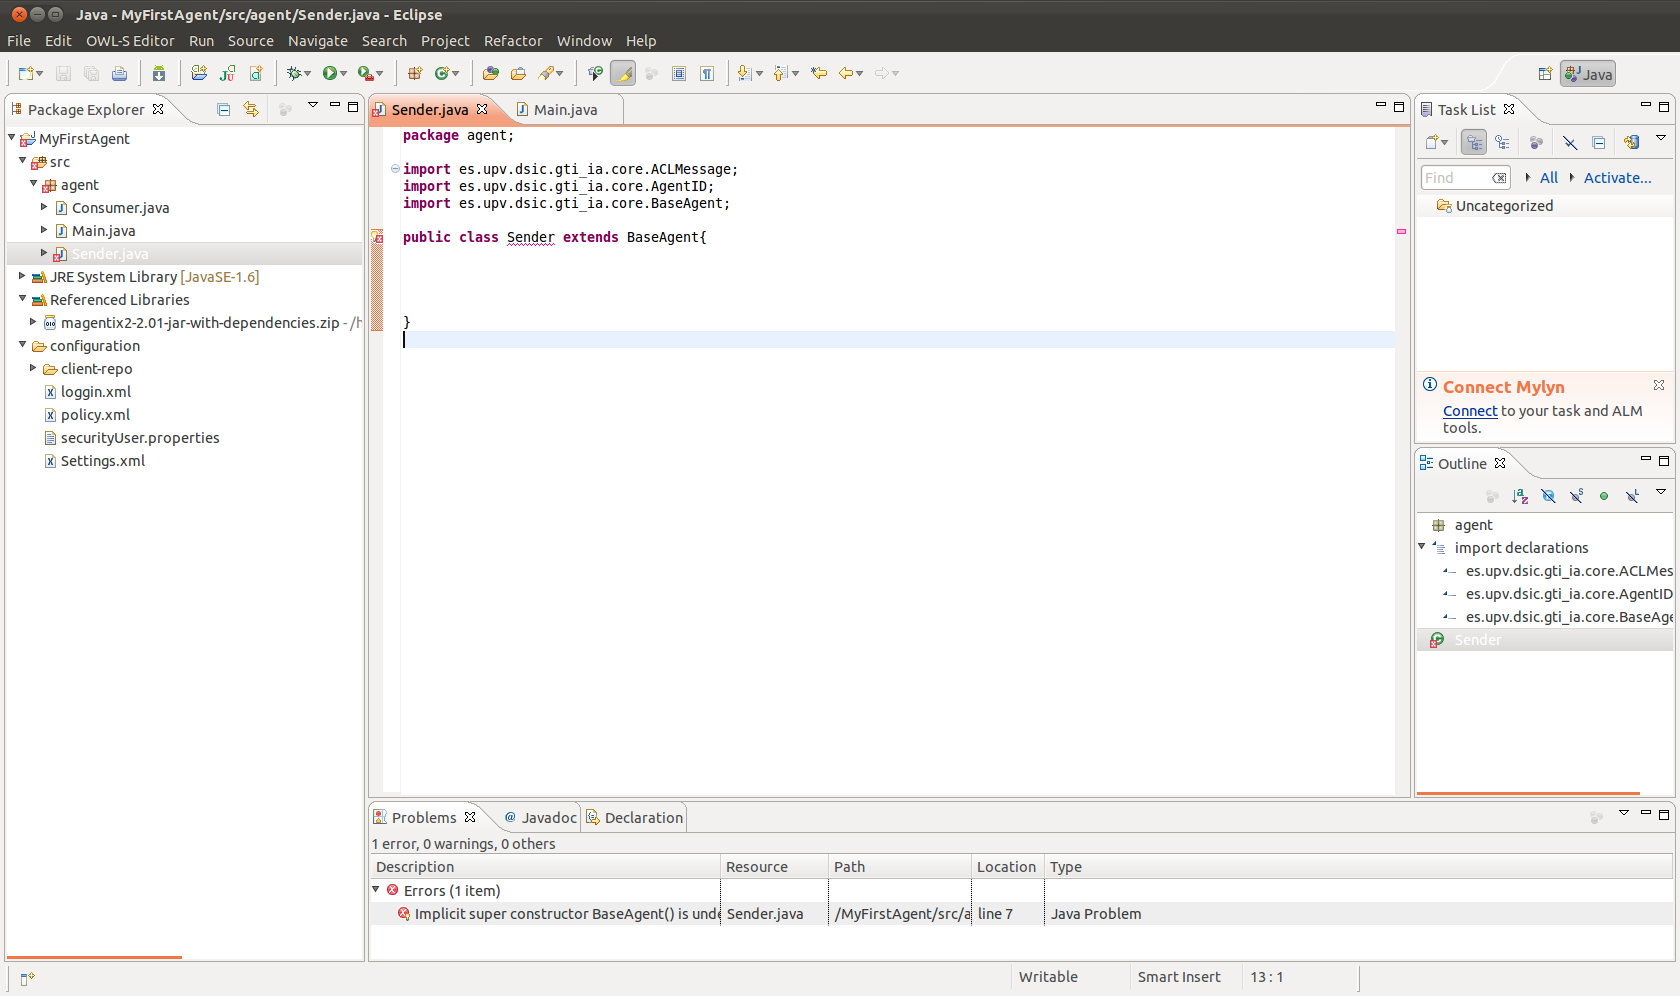
\includegraphics[scale=0.25]{Quickstart/images/develop2}
\caption{Programming a first agent with Eclipse}
\label{img:develop2}
\end{figure}



A Magentix2 agent has three main methods \texttt{init}, \texttt{execute} and \texttt{finalize}. They are executed in the cited order. In the method \texttt{init}, the code that has to be executed at the beginning of the agent execution is added. The method \texttt{execute} is the main method of the agent and \texttt{finalize} is executed just before the agent ends its execution and it is destroyed. In this specific example, it is only needed to implement code in the method \texttt{execute}. The code of the agent is shown below.
\begin{lstlisting}[style=Java]
package agent;

import es.upv.dsic.gti_ia.core.ACLMessage;
import es.upv.dsic.gti_ia.core.AgentID;
import es.upv.dsic.gti_ia.core.BaseAgent;

public class Sender extends BaseAgent {

   public Sender(AgentID aid) throws Exception {
      super(aid);
   }

   public void execute(){
      System.out.println("Hi! I'm agent "+this.getName()+" and I start my execution");
      ACLMessage msg = new ACLMessage(ACLMessage.INFORM);
      msg.setSender(this.getAid());
      msg.addReceiver(new AgentID("Consumer"));
      msg.setContent("Hi! I'm Sender agent and I'm running on Magentix2");
      this.send(msg);
   }

}
\end{lstlisting}

Following there is an explanation of all the code in the previously shown \texttt{execute} method line by line:
\begin{itemize}
   \item The agent says hello and shows its name on the console (line 14).
   \item A new ACLMessage called \textit{msg} is created (line 15). The performative of this message is \textit{Inform}.
   \item This agent (\textit{Sender} agent) is set as the sender of the message (line 16).
   \item The  \textit{Consumer} agent is added as a receiver of the agent (line 17). 
   \item The content of the message \textit{msg} is specified (line 18).
   \item Finally the agent sends the message, and with this ends its execution (line 19).
\end{itemize}
Now it is time to program the \textit{Consumer} agent. This agent will wait until it receives the message from the \textit{Sender} agent. Then it will show the content of the message on the console and it ends its execution. The code of the \textit{Consumer} agent is shown below.
\begin{lstlisting}[style=Java]
package agent;

import es.upv.dsic.gti_ia.core.ACLMessage;
import es.upv.dsic.gti_ia.core.AgentID;
import es.upv.dsic.gti_ia.core.SingleAgent;

public class Consumer extends SingleAgent{

   boolean gotMsg = false;

   public Consumer(AgentID aid) throws Exception {
      super(aid);
   }

   public void execute(){
      System.out.println("Hi! I'm agent "+this.getName()+" and I start my execution");
      ACLMessage msg = null;
      try {
	 msg = this.receiveACLMessage();
      } catch (InterruptedException e) {
	 e.printStackTrace();
      }
      System.out.println("Hi! I'm agent "+this.getName()+" and I've received the message: "+msg.getContent());
   }
}
\end{lstlisting}
This agent does not extend from BaseAgent but from SingleAgent (section \ref{sec:SimpleAgent}), this allows using the  \texttt{receiveACLMessage} method. This method halts the agent execution until it receives a message. The method \texttt{execute} of the \textit{Consumer} agent does nothing but wait until the agent receives a message. When the agent receives a message, it assigns the message to the variable \texttt{msg} and then it shows the message content on the console.

Once both agents are programmed, the Main.java class should be programmed. This class is in charge of connecting the agents to the broker and starting their execution. The code of this class is shown below.

\begin{lstlisting}[style=Java]
package agent;

import org.apache.log4j.Logger;
import org.apache.log4j.xml.DOMConfigurator;
import es.upv.dsic.gti_ia.core.AgentID;
import es.upv.dsic.gti_ia.core.AgentsConnection;

public class Main {

   public static void main(String[] args) {
      /**
      * Setting the Logger
      */
      DOMConfigurator.configure("configuration/loggin.xml");
      Logger logger = Logger.getLogger(Main.class);

      /**
      * Connecting to Qpid Broker
      */
      AgentsConnection.connect("localhost", 5672,  "test", "guest", "guest", false);


      try {
	 /**
	 * Instantiating a sender agent
	 */
	 Sender senderAgent = new Sender(new AgentID("Sender"));

	 /**
	 * Instantiating a consumer agent
	 */
	 Consumer consumerAgent = new Consumer(new AgentID("Consumer"));

	 /**
	 * Execute the agents
	 */
	 consumerAgent.start();
	 senderAgent.start();

      } catch (Exception e) {
	 logger.error("Error  " + e.getMessage());
      }
   }

}
\end{lstlisting}
In lines 14 and 15, the logger mechanism is set up. Its basic functionality is to show messages at some points of the code. This messages have a priority level associated, these levels go from info to error. It is needed to specify the configuration file for the debugger and the class to debug (Main class in this example). In line 20, the connection to the broker for all the agents launched in this class is set up. In this particuar case, it is  specified that the QPid broker is running in the same host that the agents. The other parameters are the values for a default configuration of the broker. From lines 27 to 38, the agents are created, specifying an agent id for each one, and then they are started.

If Eclipse is used, the example can be run using the run button. The result of the execution will appear on the console, and it should be something similar to what is shown below.
\begin{codigo}
Hi! I'm agent Consumer and I start my execution
Hi! I'm agent Sender and I start my execution
Hi! I'm agent Consumer and I've received the message: Hi! I'm Sender
agent and I'm running on Magentix2
\end{codigo}




